\section{Layout}

\begin{figure}[H]
    \hspace*{-2.5cm}
    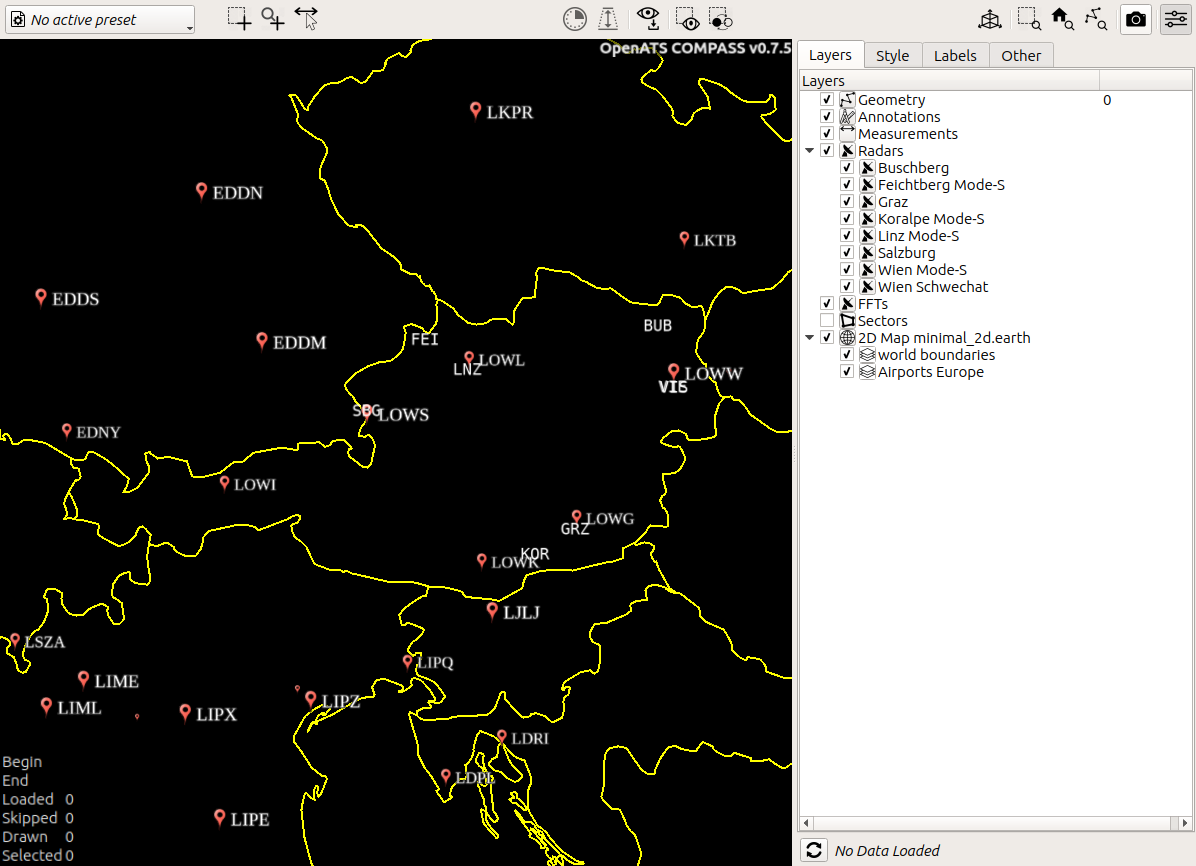
\includegraphics[width=19cm,frame]{figures/geoview_overview.png}
  \caption{Geographic View overview}
  \label{fig:geoview_overview}
\end{figure}

The map window will automatically traverse to the medium location of the data in the current database and later pan/zoom to the loaded data (on the first load only). \\

There exist 3 main components:
\begin{itemize}
 \item Toolbar (top left): Selects mouse action or set display options
 \item Data Widget (lower left): Displays map and geometry data
 \item Configuration panel (right): Allows adaption what and how geometry data is displayed
\end{itemize}
\ \\

Please note that the Data Widget and the Configuration panel can be resized and hidden if wanted. \\

To load the data use the the mechanism described in section \nameref{sec:ui_overview} can be used. To filter the dataset, the mechanism described in section \nameref{sec:filters} can be used. \\

After loading, the target reports will be shown.

\begin{figure}[H]
    \hspace*{-2.5cm}
    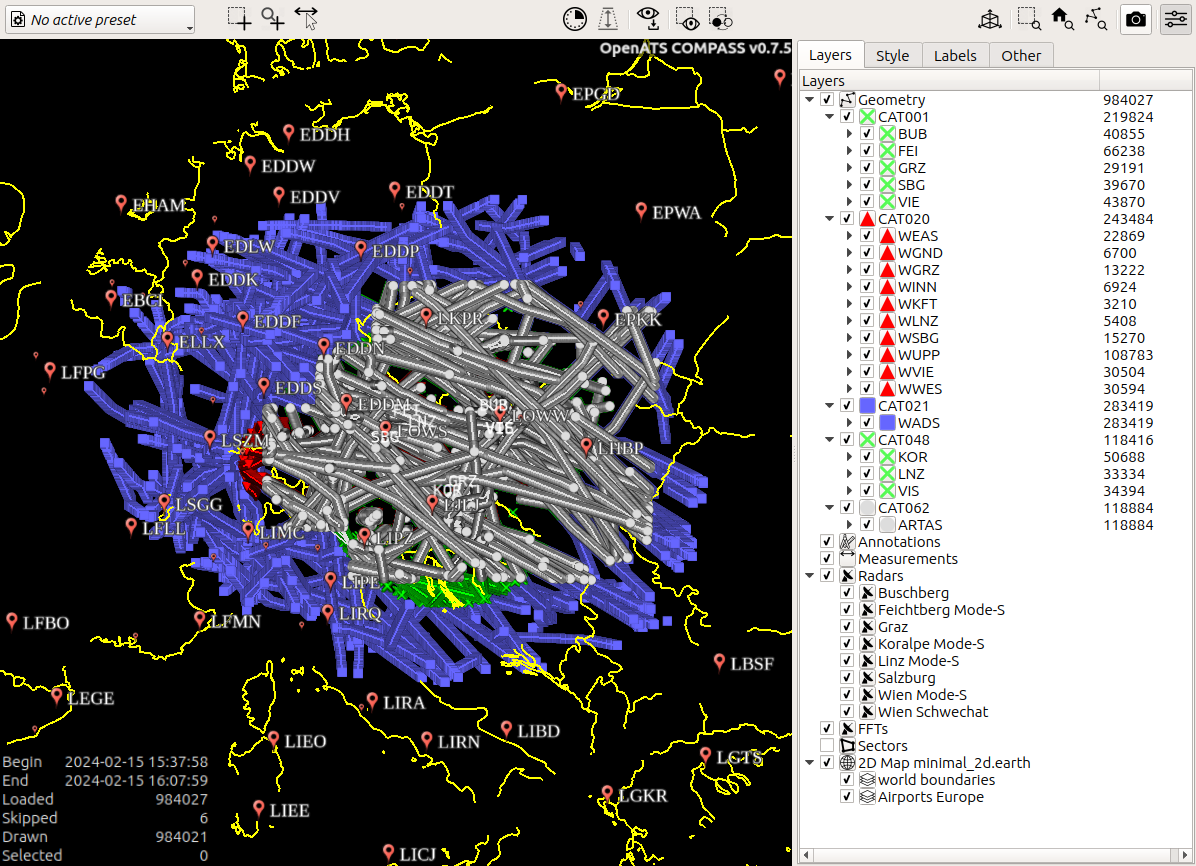
\includegraphics[width=19cm,frame]{figures/geoview_overview_loaded.png}
  \caption{Geographic View overview after loading}
\end{figure} 

How the data is presented in defined in the Configuration panel, please refer to \nameref{sec:geoview_config_panel} for details. \\

For each DSType, a default display configuration is set:

\begin{itemize}
 \item Tracker: White circle (default)
 \item Radar: Green cross (default)
 \item MLAT: Red triangle (default)
 \item ADS-B: Blue square (default)
 \item RefTraj: Orange plus-sign (default)
\end{itemize}
\ \\

There exist two display modes, 2D(default) and 3D, which are set based on the used map:

\begin{itemize}
 \item 2D: Displays map in a 2D projection and (per default) disables usage of height in geometry data drawing
 \item 3D: Displays map as a globe and (per default) enables usage of height in geometry data drawing
\end{itemize}
\ \\
Please refer to \nameref{ref:geoview_map_ops} for details.
